
\section[]{\textgreek{Πλήθος υπαλλήλων που προσλήφθηκαν το 2002 και εργάζονται σε έργα με πρόοδο $<75\%$}}


\begin{frame}[t, fragile, shrink]
\frametitle{Πρόσληψη το 2002}
\begin{block}{\small Να βρεθεί το πλήθος των υπαλλήλων που προσλήφθηκαν
μέσα στο 2002 και απασχολούνται σε έργα με βαθμό προόδου μικρότερο του 75\%}
\pause
\en
\begin{SQL}
 COUNT(DISTINCT e.empid)
------------------------
                       3
\end{SQL}
\el
\end{block}
\pause
\vspace{0.5cm}
\begin{minipage}{\wE}
\begin{enumerate} \itemsep 4pt
  \item Πληροφορίες από τον πίνακα {\ra employees}
  \item Αναζήτηση με βάση δεδομένα από τους πίνακες {\ra employees, projects}
  \item Λύση: {\crr σύζευξη πινάκων}
  \item {\crr Προσοχή} στη χρήση του πίνακα {\ra workson}
\end{enumerate}
\end{minipage}
\end{frame}


\begin{frame}[t, fragile, shrink]
\frametitle{Πρόσληψη το 2002 και πρόοδος έργων}
\begin{minipage}{\wE}
  \vspace{-0.5cm}
  \begin{block}{Ποιοι πίνακες χρειάζονται?}
    \begin{enumerate} \itemsep 6pt
      \item Στοιχεία υπαλλήλων {\ra empid, hiredate}, επομένως ο πίνακας {\sq employees}.
      \item Στοιχεία έργων: {\ra progress}, επομένως ο πίνακας {\sq projects}.
      \item Σύζευξη πινάκων υπαλλήλων και έργων, επομένως ο πίνακας {\sq workson}.
    \end{enumerate}
  \end{block}
  \vspace{0.5cm}
  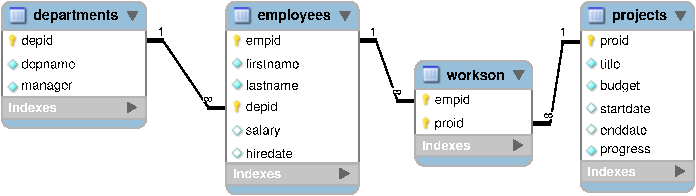
\includegraphics[scale=0.9]{../common/companyREL.pdf}
\end{minipage}
\end{frame}



\begin{frame}[t, fragile, shrink]
\frametitle{Πρόσληψη το 2002 -- βήμα 1}
\begin{minipage}{\wE}
\vspace{-0.5cm}
\begin{block}{\small Σύζευξη πινάκων}
\[
  \begin{split}
      \varrho_{e} (employees) \bowtie_{e.empid=w.empid} \varrho_{w} (workson)  \\
                              \bowtie_{w.proid=p.proid} \varrho_{p} (projects)
  \end{split}
\]
\vspace{-0.5cm}
\pause
\en
\begin{SQL}
    FROM (employees e INNER JOIN workson  w
                         ON e.empid = w.empid)
                      INNER JOIN projects p
                         ON w.proid = p.proid
\end{SQL}
\el
\end{block}
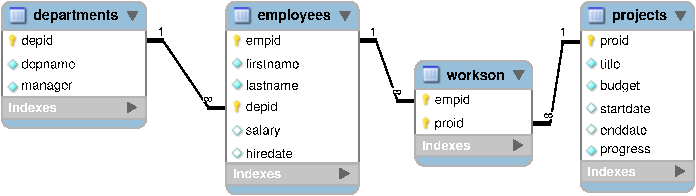
\includegraphics[scale=0.9]{../common/companyREL.pdf}
\end{minipage}
\end{frame}



\begin{frame}[t, fragile, shrink]
\frametitle{Πρόσληψη το 2002 -- βήμα 2}
\begin{minipage}{\wE}
\vspace{-0.5cm}
  \begin{block}{\small Περιορισμός εγγραφών }
Περιορισμός με βάση την ημερομηνία πρόσληψης και την πρόοδο έργου:
\[
\begin{split}
      \sigma_{\sigma_{e.hiredate\geq'2002-01-01'\wedge e.hiredate\leq'2002-12-31'}
                      \wedge p.progress>75}
      (                           \\
        \varrho_{e} (employees) \bowtie_{e.empid=w.empid} \varrho_{w} (workson) \\
                                \bowtie_{w.proid=p.proid} \varrho_{p} (projects)
      )
\end{split}
\]
\pause
\vspace{-0.5cm}
\en
\begin{SQL}
    FROM (employees e INNER JOIN workson  w
                         ON e.empid = w.empid)
                      INNER JOIN projects p
                         ON w.proid = p.proid
   WHERE e.hiredate BETWEEN '2002-01-01' AND '2002-12-31'
     AND p.progress < 75
\end{SQL}
\el
\end{block}
\end{minipage}
\end{frame}



\begin{frame}[t, fragile, shrink]
\frametitle{Πρόσληψη το 2002 -- τελική διατύπωση}
\begin{minipage}{\wE}
\vspace{-0.55cm}
  \begin{block}{\small Καταμέτρηση πλήθους}
\[
\begin{split}
    {}_{} \calg_{count(e.empid)}    
      \sigma_{\sigma_{e.hiredate\geq'2002-01-01'\wedge e.hiredate\leq'2002-12-31'}
                      \wedge p.progress>75}
      (                           \\
        \varrho_{e} (employees) \bowtie_{e.empid=w.empid} \varrho_{w} (workson)   \\
                                \bowtie_{w.proid=p.proid} \varrho_{p} (projects)
      )
\end{split}
\]
\pause
\vspace{-0.55cm}
\en
\begin{SQL}
  SELECT COUNT(DISTINCT e.empid)
    FROM (employees e INNER JOIN workson  w
                         ON e.empid = w.empid)
                      INNER JOIN projects p
                         ON p.proid = w.proid
   WHERE e.hiredate BETWEEN '2002-01-01' AND '2002-12-31'
     AND p.progress < 75;

 COUNT(DISTINCT e.empid)
------------------------
                       3
\end{SQL}
\el
\end{block}
\end{minipage}
\end{frame}


\begin{frame}[t, fragile, shrink]
\frametitle{Πρόσληψη το 2002 -- λάθος διατύπωση}
\begin{minipage}{\wE}
\vspace{-0.55cm}
\begin{alertblock}{\small Χωρίς απαλοιφή διπλοεγγραφών}
\vspace{-0.55cm}
\[
\begin{split}
    {}_{} \calg_{count(e.empid)}
      \sigma_{\sigma_{e.hiredate\geq'2002-01-01'\wedge e.hiredate\leq'2002-12-31'}
                      \wedge p.progress>75}
      (                           \\
        \varrho_{e} (employees) \bowtie_{e.empid=w.empid} \varrho_{w} (workson)   \\
                                \bowtie_{w.proid=p.proid} \varrho_{p} (projects)
      )
\end{split}
\]
\pause
\vspace{-0.55cm}
\en
\begin{SQL}
  SELECT &color{red}COUNT(e.empid) &color{black}
    FROM (employees e INNER JOIN workson  w
                         ON e.empid = w.empid)
                      INNER JOIN projects p
                         ON p.proid = w.proid
   WHERE e.hiredate BETWEEN '2002-01-01' AND '2002-12-31'
     AND p.progress < 75;

 COUNT(e.empid)
---------------
              5
\end{SQL}
\el
\end{alertblock}
\end{minipage}
\end{frame}


\begin{frame}[t, fragile, shrink]
\frametitle{Πρόσληψη το 2002 -- γιατί {\en DISTINCT}?}
\begin{minipage}{\wE}
\vspace{-0.55cm}
\begin{block}{\small Τι παρατηρείτε?}
\en
\begin{SQL}
  SELECT e.empid, e.hiredate, p.proid, p.progress
    FROM (employees e INNER JOIN workson  w
                         ON e.empid = w.empid)
                      INNER JOIN projects p
                         ON w.proid = p.proid
   WHERE e.hiredate BETWEEN '2002-01-01' AND '2002-12-31'
     AND p.progress < 75;

 empid  hiredate    proid  progress
------------------------------------
   206  2002-12-03     12      60.0
   230  2002-12-03     12      60.0
   230  2002-12-03     14      20.0
   431  2002-09-16     14      20.0
   230  2002-12-03     38       0.0
\end{SQL}
\el
\end{block}
\end{minipage}
\end{frame}


\begin{frame}[t, fragile, shrink]
\frametitle{Διαχωρισμός δύο εννοιών}
\begin{minipage}{\wE}
\pause
\vspace{-0.7cm}
\begin{alertblock}{\small Πλήθος συμμετοχών υπαλλήλων σε έργα}
\en
\begin{SQL}
  SELECT COUNT(e.empid)
    FROM (employees e INNER JOIN workson  w
                         ON e.empid = w.empid)
                      INNER JOIN projects p
                         ON w.proid = p.proid
   WHERE e.hiredate BETWEEN '2002-01-01' AND '2002-12-31'
     AND p.progress < 75;
\end{SQL}
\el
\end{alertblock}
\pause
\vspace{-0.7cm}
\begin{exampleblock}{\small Πλήθος υπαλλήλων που απασχολούνται σε έργα}
\en
\begin{SQL}
  SELECT COUNT(DISTINCT e.empid)
    FROM (employees e INNER JOIN workson  w
                         ON e.empid = w.empid)
                      INNER JOIN projects p
                         ON w.proid = p.proid
   WHERE e.hiredate BETWEEN '2002-01-01' AND '2002-12-31'
     AND p.progress < 75;
\end{SQL}
\el
\end{exampleblock}  
\end{minipage}
\end{frame}

